\documentclass[a4paper,twocolumn]{article}

\usepackage[T1]{fontenc}
\usepackage{lmodern}
 \usepackage{amsmath}
 \RequirePackage[nottoc]{tocbibind}

% Paket za hrvatski jezik neispravno izostavlja toèke iza naslova,
% to ispravljamo zadavanjem novih funkcija za numeriranje koje stavljaju
% toèku.
\makeatletter
\renewcommand\thesection{\@arabic\c@section.}
\renewcommand\thesubsection{\thesection\@arabic\c@subsection.}
\renewcommand\thesubsubsection{\thesubsection\@arabic\c@subsubsection.}
\renewcommand\theequation{\@arabic\c@equation}
\renewcommand\thefigure{\@arabic\c@figure.}
\renewcommand\thetable{\@arabic\c@table.} 
\makeatother

% Ostali korisni paketi.
\RequirePackage{graphicx}
\RequirePackage{hyperref}
\RequirePackage{amssymb}
\RequirePackage{amsmath}
\usepackage{subcaption}
\usepackage{float}
\usepackage{todonotes}

\bibliographystyle{plain}

\usepackage[croatian]{babel}




% Ovdje zapoèinje èlanak.
\begin{document}
	
	% Navedite naslov i autore. Datume se automatski postavlja na datum kreiranja dokumenta,
	% no može se promijeniti zadavanjem \date{30. veljaèe, 2004.}
	\title{Paralelna realizacija metoda za obradu slike pomoću NVIDIA CUDA tehnologije} 
	\author{Marko Haralović, Ita Poklepović, Lana Barić, Dino Babić,  Anabel Dautović, Valeria Javornik}
	\maketitle

	
	\section*{Sažetak}
	U ovom radu analizirana je razlika u performansi između centralnih procesorskih jedinica (CPU) i grafičkih procesorskih jedinica (GPU) prilikom izvršavanja nekih od odabranih metoda obrade slika koristeći CUDA tehnologiju.  Ukratko će biti opisana teoretska razlika između funkcionalnosti CPU i GPU, a onda objašnjena i prikazana implementacija odabranih metoda za koju su korištene Numpy, Cupy i scikit-image open-source python biblioteke. Korištene metode odabrane su zbog svoje važnosti u području obrade digitalnih slika, a uključuju matrično množenje, detekciju rubova pomoću Sobel i Canny operatora, grupiranje s K srednjim vrijednostima, treniranje neuronske mreže za klasifikaciju rukom pisanih znamenaka, te ostale metode koje će kasnije biti predstavljene. Eksperimenti pokazuju da razlike u kvaliteti rezultata između CPU i GPU nema, ali u brzini izvođenja metoda, GPU je i do 10 puta veći.
 
	
	\section{Uvod}
	
    Područje obrade slika obuhvaća mnoge tehnike i metode za manipulaciju i analizu slika, koje se koriste za različite primjene u gotovo svim disciplinama. U ovom radu, fokus je na obradi informacija gdje je ulazni signal digitalna slika prikazana kao dvodimenzionalna matrica s jednim kanalom (slika bez boje - siva vrijednost) ili s tri kanala (slika u boji - RGB kanali). \newline
    Obrada slika je izuzetno važna zbog svoje široke primjene u mnogim područjima. Na primjer, koristi se za olakšavanje medicinske dijagnostike, industrijske automatizacije, forenzike, autonomnih vozila, poljoprivrede, geografije, građevine i mnogih drugih disciplina. Široka primjenjivost ovog područja zahtjeva da korištene metode budu ne samo točne, već i efikasne u pogledu korištenja resursa. U računarstvu, cilj je često da se metode izvode što brže, ali pritom treba uzeti u obzir i trošak bržeg izvođenja, posebno kada se ubrzanje postiže unapređenjem fizičke arhitekture računala.
    
	
	\section{GPU, CPU i aktivnost u svijetu}

        Grafički procesori (GPU) prvo su se počeli koristiti za poboljšanje performansi videoigara. Već 1970-ih godina, u arkadne igre su se ugrađivali posebni čipovi čiji je zadatak bio prikazivanje videoigre na ekranu. Međutim, trebalo je dugo vremena da se GPU-ovi počnu šire koristiti za ubrzavanje drugih procesa.
        
        CPU (centralna procesorska jedinica) i GPU općenito se razlikuju u svojoj arhitekturi i primjeni. CPU se sastoji od manjeg broja jezgri (najčešće od 2 do 16), što ograničava njegovu sposobnost za istovremeno izvršavanje zadataka. Kada se zadaci paraleliziraju na CPU-u, koriste se njegove jezgre, no zbog malog broja jezgri, samo se nekoliko zadataka može izvršavati istovremeno. Često se koristi prividna paralelizacija gdje se više zadataka brzo prebacuje s jedne jezgre na drugu. Ovakva paralelizacija nije najefikasnija jer je promjena konteksta dretvi vremenski neučinkovita.
        
        S druge strane, GPU se sastoji od velikog broja jezgri, koje u boljim grafičkim karticama mogu brojati desetke tisuća. Ovo ga čini idealnim za paralelno izvođenje velikog broja jednostavnih operacija. Na slici \ref{fig:cpu_vs_gpu} može se vidjeti razlika u arhitekturi dviju procesorskih jedinica.
        
        \begin{figure}[H]
        	\centering
        	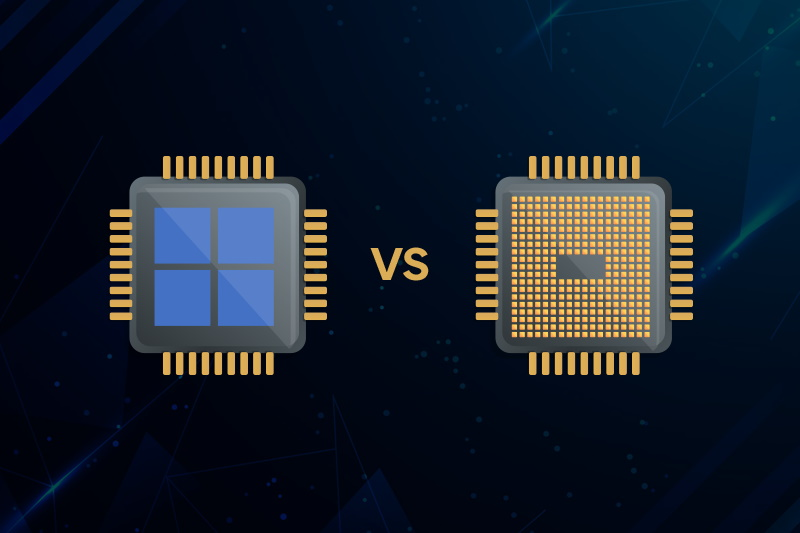
\includegraphics[width=0.7\linewidth]{slike/CPU-vs-GPU.jpg}
        	\caption{Pojednostavljeni prikaz CPU (lijevo) i GPU (desno) \cite{GPUvsCPU}}
        	\label{fig:cpu_vs_gpu}
        \end{figure}
        
        Trenutno je NVIDIA vodeća tvrtka u razvoju GPU tehnologije. Osnovana je 1993. godine, a svoju popularnost stekla je lansiranjem prvog grafičkog procesora, nazvanog GeForce. CUDA je također tehnologija koju je razvila NVIDIA, a omogućuje programerima da pišu kod i pritom koriste funkcije koje će se izvršavati paralelno, na grafičkom procesoru.
        
        \section{Prijenos podataka između CPU i GPU}
        
        Prijenos podataka s CPU na GPU je vremenski zahtjevan. Da bi korištenje GPU-a doista bilo isplativo, potrebno je baratati s velikom količinom podataka. Ako je podataka malo, tada će CPU obaviti istu operaciju brže nego li GPU, upravo zbog prijenosa podataka na GPU. Na slici \ref{fig:data_to_gpu} prikazana su vremena prijenosa matrica na GPU. Najmanja matrica je veličine 100x100, a najveća veličine 20000x20000. 
        
        \begin{figure}[H]
        	\centering
        	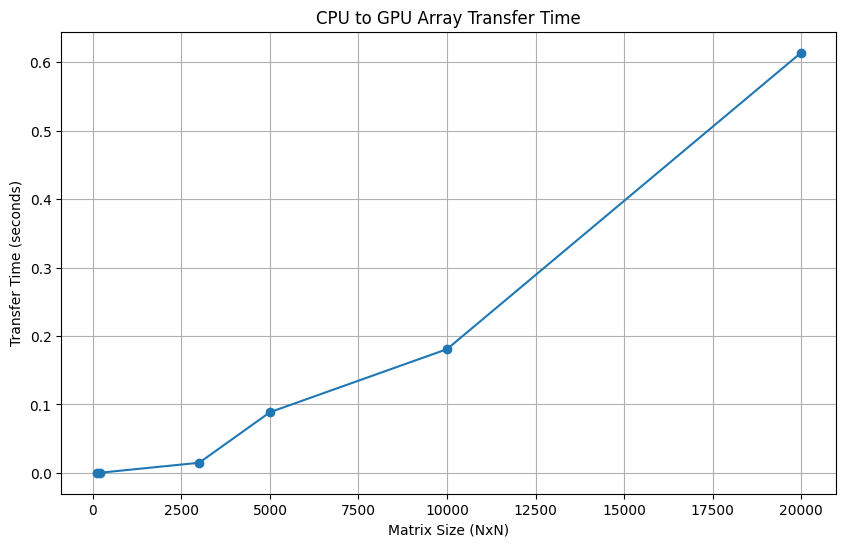
\includegraphics[width=0.9\linewidth]{slike/data_to_gpu.png}
        	\caption{Prikaz vremena prijenosa matrica različitih veličina na GPU.}
        	\label{fig:data_to_gpu}
        \end{figure}
        
	\section{Pregled implementiranih metoda za obradu slika pomoću NVIDIA CUDA tehnologije}
	
	\subsection{Usporedba matričnog množenja na CPU i GPU te primjena nad transformacijama slike}
	
		Matrično množenje vrlo je često korištena operacija te je nužno osigurati njezino učinkovito izvođenje čak i u slučaju vrlo velikih matrica. Razmotrimo sljedeći primjer. Kreirane su kvadratne matrice veličina od 150x150 do 1500x1500. Svaka matrica pomnožena je sama sa sobom te je vrijeme obavljanja te operacije zabilježeno. Na slici \ref{fig:cpu_gpu_comparison} prikazana su vremena izvođenja u slučaju korištenja CPU-a i u slučaju korištenja GPU-a. Na slici možemo uočiti da je izvođenje značajno brže na GPU, čak i za relativno male veličine matrica.
		
		\begin{figure}[H]
			\centering
			\begin{subfigure}{0.45\textwidth}
				\centering
				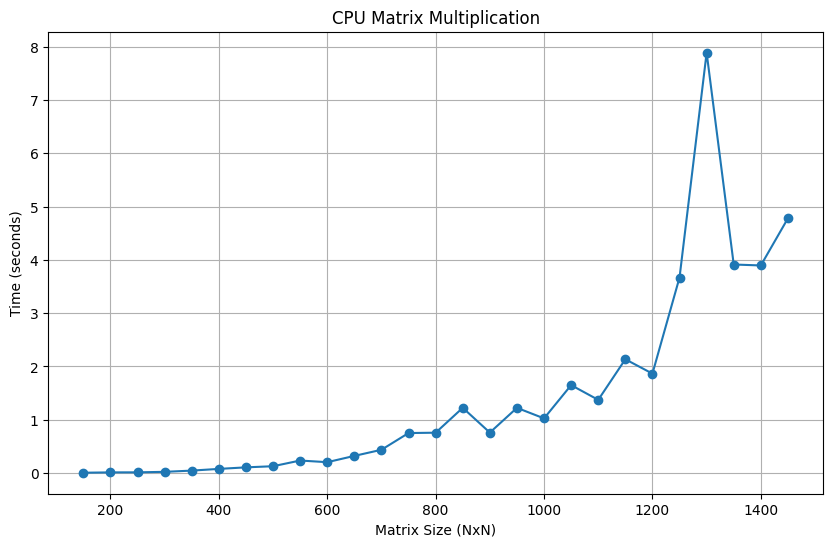
\includegraphics[width=\linewidth]{slike/cpu_mat_mul.png}
				\caption{Vrijeme izvođenja na CPU.}
			\end{subfigure}
			\hfill
			\begin{subfigure}{0.45\textwidth}
				\centering
				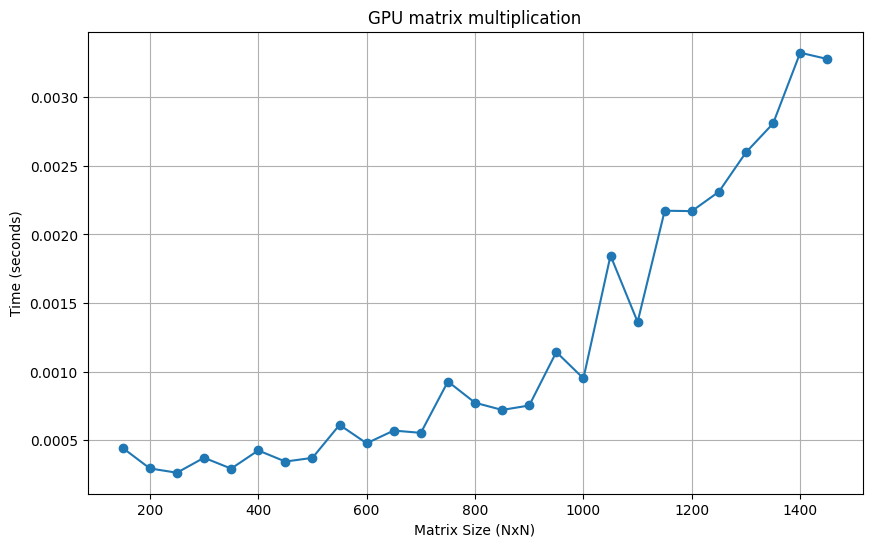
\includegraphics[width=\linewidth]{slike/gpu_mat_mul.png}
				\caption{Vrijeme izvođenja na GPU.}
			\end{subfigure}
			\caption{Usporedba vremena množenja matrica na CPU i GPU.}
			\label{fig:cpu_gpu_comparison}
		\end{figure}

        \subsection{Linearna geometrijska transformacija}

        Linearne geometrijske transformacije slika ukljućuju translaciju, skaliranje i rotaciju. Prikazana matrica transformacije rotacije (\ref{eq:rotation}) određuje koja je nova pozicija jednog pixela slike. Ova je metoda savršen primjer za paralelizaciju jer je račun nove pozicije svakog pixela u potpunosti neovisan o ostalima pa se teoretski mogu svi računati u isto vrijeme. Naravno to neće uvjek biti moguće zbog ograničenog broja jezgri GPU-a.
        
               \begin{equation}
                    \begin{bmatrix}
                    x \\
                    y \\
                    1
                    \end{bmatrix}
                    =
                    \begin{bmatrix}
                    \cos \theta & -\sin \theta & 0 \\
                    \sin \theta & \cos \theta & 0 \\
                    0 & 0 & 1
                    \end{bmatrix}
                    \begin{bmatrix}
                    u \\
                    v \\
                    1
                    \end{bmatrix}
                    \label{eq:rotation}
                \end{equation}

        Na slici \ref{fig:rotation_results} je vidljivo da paralelizaciju pomoću GPU-a nikako ne utječe na ispravnost transformacije, ali zato kao što je vidljivo iz grafa \ref{fig:tranformatoin_timming} znatno utječe na brzinu jer se koristeći CPU pozicija svakog piksela treba slijedno računati. Korištena slika je veličine 1024 x 1024 i rotirana je za 45$^\circ$.

        \begin{figure}[H]
		\centering
		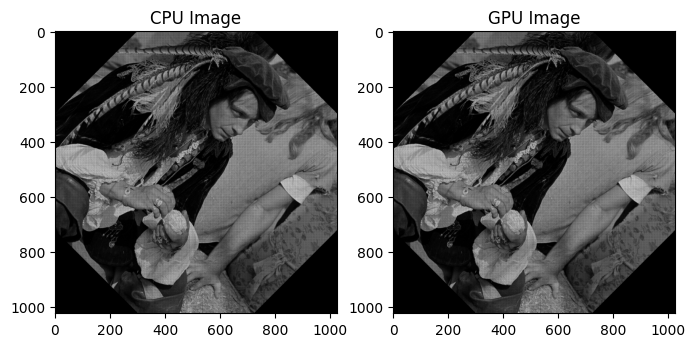
\includegraphics[width=0.9\linewidth]{slike/img_tranformation_results.png} 
		\caption{Rezultati rotacije računate na CPU i GPU}
		\label{fig:rotation_results}
	\end{figure} 

        \begin{figure}[H]
		\centering
		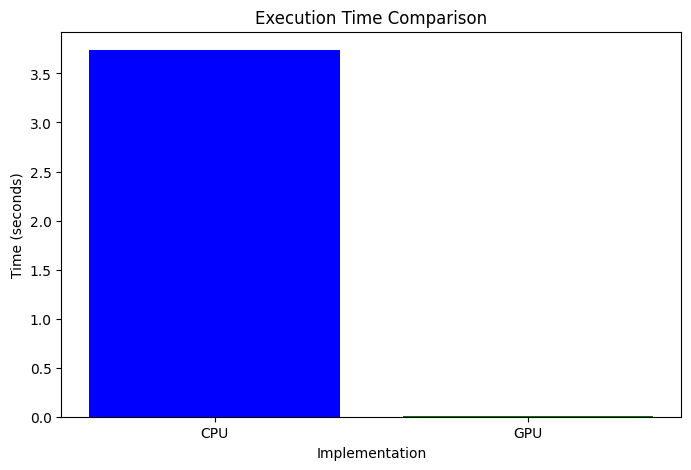
\includegraphics[width=0.9\linewidth]{slike/image_tranformatoin_timming_graph.png} 
		\caption{Razlika u vremenu izvođenja transformacije rotacije na CPU (3.738 s) i GPU (0.005 s)}
		\label{fig:tranformatoin_timming}
	\end{figure} 

        \subsection{Sobel operator za detekciju rubova}
        Sobel operator jedan je od poznatijih algoritama za detekciju rubova u slikama. Za aproksimaciju prve derivacije intenziteta slike koristi dvije matrice veličine 3x3.
        \[
        G_x = \begin{bmatrix}
        	-1 & 0 & +1 \\
        	-2 & 0 & +2 \\
        	-1 & 0 & +1 
        \end{bmatrix}
        \quad \text{i} \quad
        G_y = \begin{bmatrix}
        	-1 & -2 & -1 \\
        	0 & 0 & 0 \\
        	+1 & +2 & +1 
        \end{bmatrix}
        \]
        
        Izradili smo dvije implementacije Sobel operatora, jednu koristeću biblioteku NumPy i drugu koristeći biblioteku CuPy koja omogućava izvođenje na GPU.
        Na slici \ref{fig:sobel_comparison} prikazana je usporedba vremena izvoženja Sobel implementacije koja se izvodi na GPU i one koja se izvodi na CPU.
        
        \begin{figure}[H]
        	\centering
        	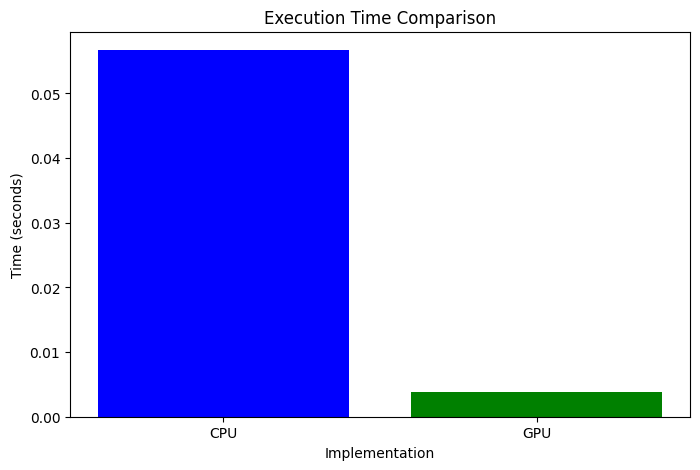
\includegraphics[width=0.9\linewidth]{slike/sobel_comparison.png} 
        	\caption{Implementacija Sobel operatora koja se izvodi na GPU značajno je brža od one koja se izvodi na CPU.}
        	\label{fig:sobel_comparison}
        \end{figure} 
        
        
        
	\subsection{Detekcija rubova koristeći Canny detektor}
	
	Iako je Canny detektor rubova John F. Canny predstavio još u 1986. u članku \cite{Canny} on je i dan danas ostao jedan od najpouzdanijih algoritama detekcije rubova u slikama. 
	
	Canny detektor radi u više koraka. Prvi korak je redukcija šuma korištenjem Gaussovog filtra koji blago zamagljuje sliku kako bi se umanjio efekt nasumičnog šuma. Nakon uklanjanja šuma koristi se Sobel operator (objašnjen u prošlom poglavlju) kako bi se izračunao intezitet promjene vrijednosti piksela slike i njen smjer. Ovaj način detekcije rubova vraća dosta neodređene rubove pa u sljedećem koraku Canny detektor njih stanjuje eliminirajući sve piksele koji se ne nalaze na lokalnom maksimumu u pravcu gradijenta što rezultira preciznijim rubovima. Kako bi se dalje izbacili rubovi koji su potencijalno nastali zbog šuma ili varijacije koriste se dva praga: visoki i niski. Dalje se gledaju pikseli rubova. Ako je gradijent piksela manji od niskog praga odbacuje se. Ako je veći od visokog praga označuje se kao jaki rub, dok se ostali pikseli rubova označuju kao slabi rub.
	
	U zadnjem koraku se izbacuju pikseli slabih rubova u slučaju kada se ne mogu povezati s jakim rubom.
	
	Na slikama ispod mogu se vidjeti originalna slika \ref{fig:canny_original}, dobiveni rezultat Canny detektora na CPU i GPU \ref{fig:canny_CPU_GPU}.
	
	\begin{figure}[H]
		\centering
		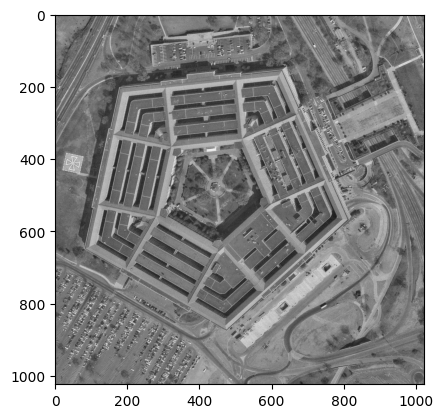
\includegraphics[width=0.9\linewidth]{slike/canny_original.png} 
		\caption{Originalna slika dimenzija 1024 x 1024}
		\label{fig:canny_original}
	\end{figure} 
	
	\begin{figure}[hbt]
		\centering
		\begin{subfigure}[]{0.49\linewidth}
			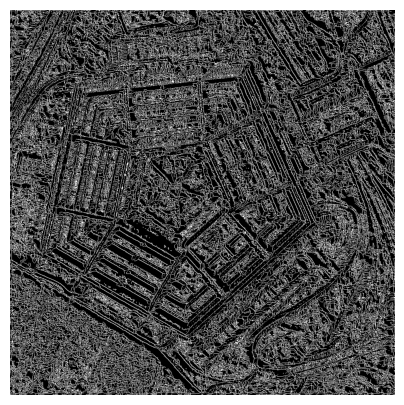
\includegraphics[width=1\linewidth]{slike/canny_np.png}
			\caption{CPU (4.807 s)}
			
		\end{subfigure}
		\begin{subfigure}[]{0.49\linewidth}
			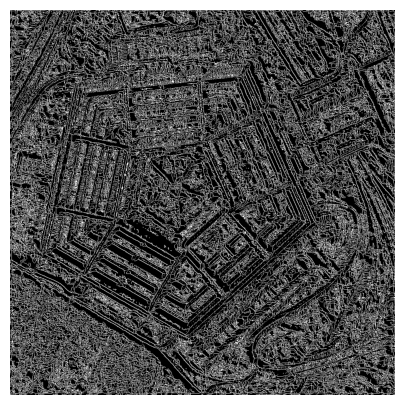
\includegraphics[width=1\linewidth]{slike/canny_cp.png}
			\caption{GPU (0.028 s)}
			
		\end{subfigure}
		\caption{Rezultati Canny detektora rubova nad slikom \ref{fig:canny_original}}
		\label{fig:canny_CPU_GPU}
	\end{figure}
	
	Na slici \ref{fig:canny_timing} vidi se razlika između vremena potrebnog za izvođenje funkcije na CPU i GPU ovisno o veličini slike koju procesiramo. Možemo vidjeti da se manje slike do otprilike 500 x 500 veličine zapravo ne isplati prebacivati na GPU, ali zato sa sve većim slikama brzina računanja na CPU raste s veličinom slike dok na GPU jedva primijeti razlika za slike veličine od čak 5000 x 5000.
	
	\begin{figure}[H]
		\centering
		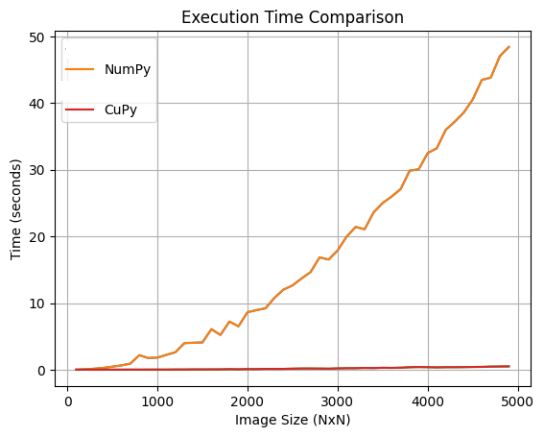
\includegraphics[width=1\linewidth]{slike/canny_timing.png} 
		\caption{Usporedba CPU i GPU izvedbe Canny detektora u ovisnosti o veličini slike}
		\label{fig:canny_timing}
	\end{figure}
        
 

        \subsection{Implementacija algoritma grupiranje s K srednjih vrijednosti za segmentaciju slike}
        
        Grupiranje s K srednjih vrijednosti ili K-means grupiranje (engl. K-means clustering) najjednostavniji je i najpoznatiji algoritam grupiranja. Algoritam ima složenost O(KnT), gdje je K broj grupa (engl. cluster), n broj podataka (u slučaju analize slika to je broj piksela), a T broj iteracija algoritma. U kodu je broj iteracija predstavljen varijablom \textit{attempts}.
        
        Ovaj postupak pripada segmentaciji grupiranjem (engl. clustering segmentation methods). K predstavlja broj (čvrstih) grupa u koje se pikseli grupiraju na temelju sličnosti. Svaka grupa ima srednju vrijednost (centroid) kojom je predstavljena.
        
        Algoritam započinje nasumičnim odabirom K centroida, nakon čega se izračunava udaljenost između svakog piksela i centroida pomoću njihovih HSV vrijednosti. Pikseli se dodjeljuju grupi najbližeg centroida. Zatim izračunava novu srednju vrijednost grupe i tu vrijednost postavlja kao centroid, nakon čega ponovno računa udaljenost svakog piksela do novo izračunatih centroida. Taj se postupak ponavlja sve dok se ne dogodi da ni jedan piksel nije promijenio grupu kojoj pripada nakon izračuna udaljenosti. 
        Algoritam se ponavlja zadani broj puta T i odabire pokušaj s najuravnoteženijom varijacijom između grupa.
        
        \begin{figure}[H]
        	\centering
        	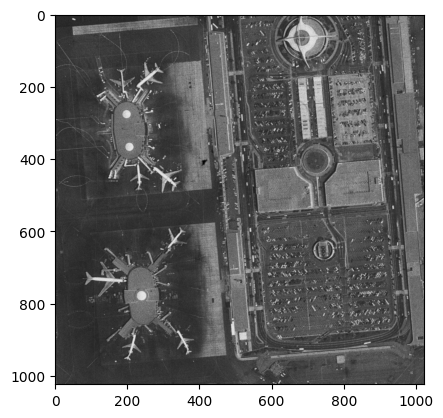
\includegraphics[width=1\linewidth]{slike/k_means_original.png} 
        	\caption{Originalna slika dimenzija 1024 x 1024}
        	\label{fig:k_means_original}
        \end{figure} 
        
        \begin{figure}[hbt]
        	\centering
        	\begin{subfigure}[]{0.49\linewidth}
        		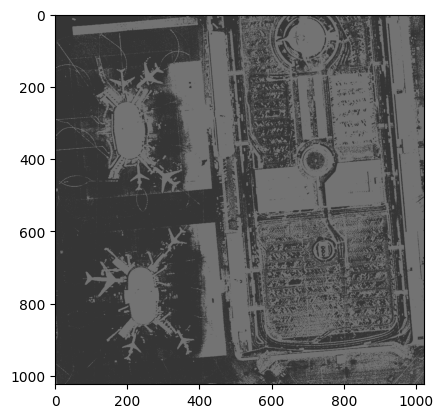
\includegraphics[width=1\linewidth]{slike/k_means_cpu.png}
        		\caption{CPU (20.013 s)}
        		
        	\end{subfigure}
        	\begin{subfigure}[]{0.49\linewidth}
        		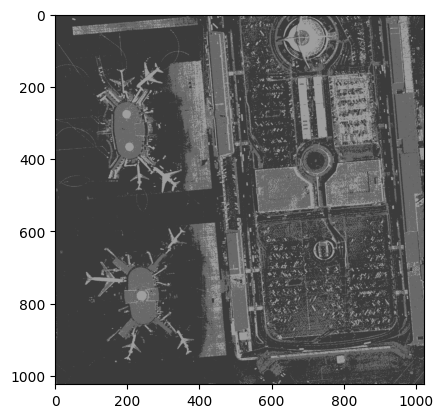
\includegraphics[width=1\linewidth]{slike/k_means_gpu.png}
        		\caption{GPU (0.795 s)}
        		
        	\end{subfigure}
        	\caption{Rezultati K-means grupiranja nad slikom \ref{fig:k_means_original}}
        	\label{fig:k_means_CPU_GPU}
        \end{figure}
        
        Rezultati grupiranja se vide na slikama \ref{fig:k_means_CPU_GPU}, a vremena provođenja metode u odnosu na veličinu slika se mogu vidjeti na slici \ref{fig:k_means_timing}. S time da inicijalne centroide generiramo nasumično vidljive su manje promjene u rezultatima. Iz rezultata mjerenja vidimo da je k-means grupiranje jako povoljna metoda za paralelizaciju. Različite jezgre GPU-a mogu biti zadužene za izračunavanje udaljenosti između jednog podatka i svih centroida i paralelno se mogu ažurirati centroide.
        
        \begin{figure}[H]
        	\centering
        	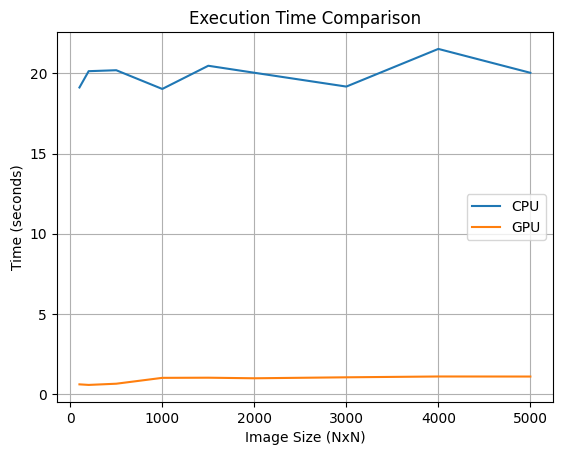
\includegraphics[width=1\linewidth]{slike/k_means_timing.png} 
        	\caption{Usporedba CPU i GPU izvedbe K-means grupiranja u ovisnosti o veličini slike}
        	\label{fig:k_means_timing}
        \end{figure}
	
	\subsection{Implementacija neuronske mreže za klasifikaciju rukom pisanih znamenaka}

	U ovom poglavlju razmotrit ćemo implementaciju neuronske mreže za klasifikaciju rukom pisanih brojeva. \cite{neural_networks} Obje implementacije napisane su u programskom jeziku Python. Verzija koja se izvodu na CPU zasniva se na biblioteci NumPy, dok se verzija koja se izvodi na GPU zasniva na biblioteci CuPy. \newline
	Za treniranje modela korišten je MNIST skup podataka, koji sadrži 60,000 slika rukom pisanih znamenaka. Svaka slika je veličine 28x28 piksela. Prilikom učitavanja skupa podataka, slike su povećane na veličinu 128x128 piksela jer je originalna veličina slika premala da bi se uočile prednosti izvođenja na grafičkim karticama. Naime, treniranje modela s originalnom veličinom slika bilo je sporije na grafičkoj kartici nego na procesoru. Iako se matrične operacije daleko brže izvode na grafičkim karticama, prenošenje podataka na grafičku karticu vremenski je skupo. U slučaju kada imamo malo podataka, vremenski je isplativije izvršiti operacije na procesoru nego prenositi podatke na grafičku karticu i natrag. \newline
	Model u ulaznom sloju ima 16,384 neurona. Skriveni sloj sadrži 30 neurona, dok izlazni sloj ima 10 neurona jer toliko imamo mogućih klasa. Za treniranje modela koristili smo stohastički gradijentni spust, dok smo kao aktivacijsku funkciju koristili sigmoidnu funkciju.
	Oba modela trenirali smo 10 epoha te su im točnosti na testnom skupu podataka bile približno jednake. Treniranje modela koji se izvršavao na procesoru je trajalo 1145 sekundi, dok je treniranje modela koji se izvršavao na grafičkoj kartici trajalo 67 sekundi. Grafička usporedba prikazana je na slici \ref{fig:cnn_training_time_comparison}. \newline
	Vremenska ušteda je značajna. Verzija modela koja se izvršava na grafičkoj kartici također radi brže predikcije, te predikciju za istu sliku izvršava gotovo deset puta brže nego model koji se izvršava na procesoru.
	
	\begin{figure}[H]
		\centering
		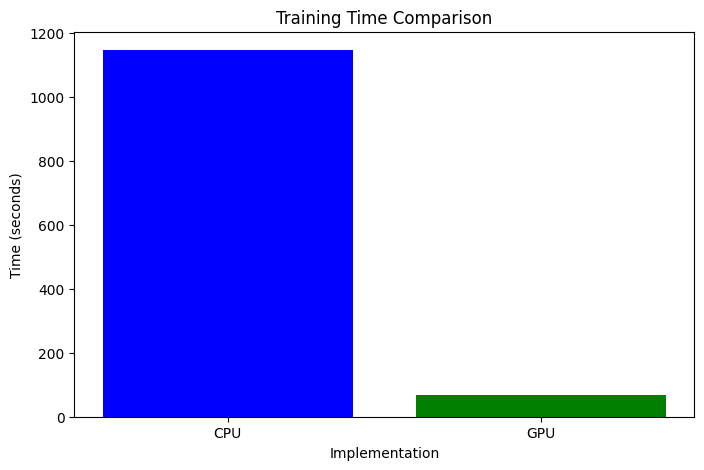
\includegraphics[width=1\linewidth]{slike/cnn_training_time_comparison.png} 
		\caption{Prikaz usporedbe vremena treniranja modela koji se izvršavaju na procesoru i na grafičkoj kartici.}
		\label{fig:cnn_training_time_comparison}
	\end{figure} 

        \subsection{Ostale metode obrade slika}
        
        Na slici \ref{fig:ostale_metode} uspoređena su vremena izvođenja na CPU i na GPU Fourierove transformacije, inverzne Fourierove transformacije, Valćine transformacije, konvolucije, uklanjanja šuma, registracija slika, računanja prosječne vrijednosti i standardne devijacije. Takođjer je zapisan broj slika na kojima se izršilo mjerenje.
        
		\begin{figure}[H]
			\centering
			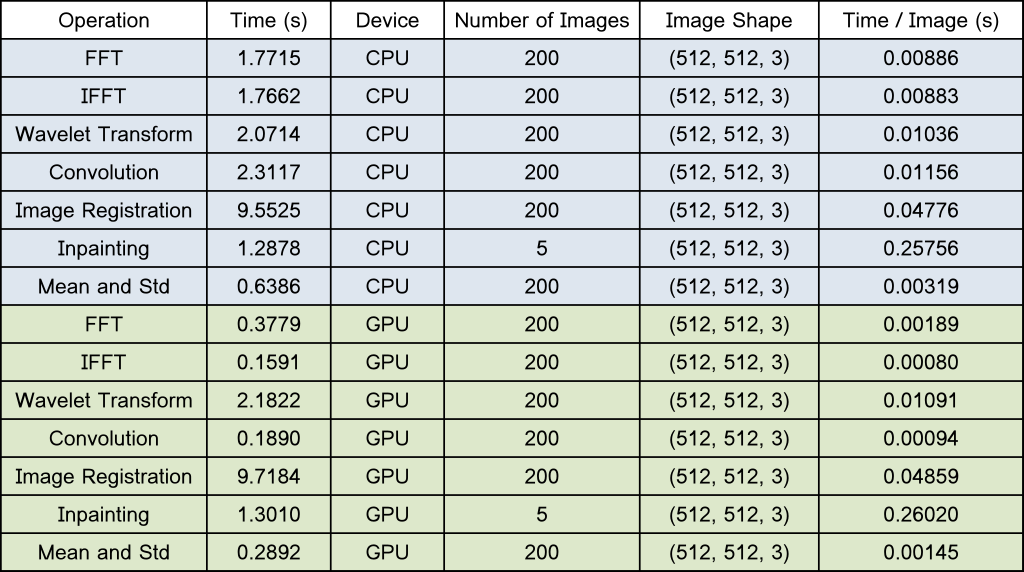
\includegraphics[width=1.05\linewidth]{slike/times_other.png} 
			\caption{Za svaku metodu tablica prikazuje vrijeme izvođenja na CPU i na GPU.}
			\label{fig:ostale_metode}
		\end{figure} 
				
	\section{Zaključak}
	Ovaj rad je detaljno analizirao razlike u performansama između centralnih procesorskih jedinica (CPU) i grafičkih procesorskih jedinica (GPU) prilikom izvršavanja različitih metoda obrade slike koristeći NVIDIA CUDA tehnologiju. Prikazane su brojne implementacije algoritama za obradu slike, kao i implementacija neuronske mreže za klasifikaciju rukom pisanih brojeva. U svim slučajevima, implementacije koje su se izvodile na GPU nadmašile su one koje su se izvodile na CPU u pogledu brzine izvršavanja. \newline
	S obzirom na to da nas u budućnosti očekuje daljnji napredak grafičkih procesora i popratnih tehnologija, gotovo je sigurno da će s vremenom postupci obrade slike biti nezamislivi bez grafičkih procesora. GPU-ovi su pokazali izuzetnu efikasnost, naročito kod obrade velikih skupova podataka i složenih algoritama, što ih čini neophodnim za napredne aplikacije u medicini, industriji, forenzici, autonomnim vozilima i drugim disciplinama. \newline
	Buduća istraživanja mogla bi biti usmjerena na analizu prijenosa podataka između CPU-a i GPU-a te na potencijalna ubrzanja tog neizbježnog dijela.
	
	
	
	% Literatura se automatski generira iz zadane liste. Svaki od elemenata liste
	% zapoèinje s oznakom, npr. \bibitem{davies}. U tekstu se referenca na èlanak
	% ili knjigu dobiva s \cite{davies}.

        \bibliography{literatura}

 
	
\end{document} 
